\documentclass[12pt,letterpaper]{article}
\usepackage{fullpage}
\usepackage[top=2cm, bottom=4.5cm, left=2.5cm, right=2.5cm]{geometry}
\usepackage{amsmath,amsthm,amsfonts,amssymb,amscd}
\usepackage{lastpage}
\usepackage{enumerate}
\usepackage{fancyhdr}
\usepackage{mathrsfs}
\usepackage{xcolor}
\usepackage{graphicx}
\usepackage{listings}
\usepackage{hyperref}

\definecolor{dkgreen}{rgb}{0,0.6,0}
\definecolor{gray}{rgb}{0.5,0.5,0.5}
\definecolor{mauve}{rgb}{0.58,0,0.82}

\lstset{frame=tb,
  language=bash,
  aboveskip=3mm,
  belowskip=3mm,
  showstringspaces=false,
  columns=flexible,
  basicstyle={\small\ttfamily},
  numbers=none,
  numberstyle=\tiny\color{gray},
  keywordstyle=\color{blue},
  commentstyle=\color{dkgreen},
  stringstyle=\color{mauve},
  breaklines=true,
  breakatwhitespace=true,
  tabsize=3
}

\hypersetup{%
  colorlinks=true,
  linkcolor=blue,
  linkbordercolor={0 0 1}
}

\lstdefinestyle{Python}{
    language        = Python,
    frame           = lines, 
    basicstyle      = \footnotesize,
    keywordstyle    = \color{blue},
    stringstyle     = \color{green},
    commentstyle    = \color{red}\ttfamily
}

\setlength{\parindent}{0.0in}
\setlength{\parskip}{0.05in}

% Edit these as appropriate
\newcommand\course{EECS 473}
\newcommand\hwnumber{3}                  % <-- homework number
\newcommand\NetIDa{ethan.shafer, ehs70}           % <-- NetID of person #1
\newcommand\NetIDb{naomi.hourihane, jdh156}        % <-- NetID of person #2 (Comment this line out for problem sets)
\newcommand\NetIDc{honglei.huo, hxh368}
\newcommand\packagename{lab3\_package}

\pagestyle{fancyplain}
\headheight 35pt
\lhead{\NetIDa\\\NetIDb\\\NetIDc}                 % <-- Comment this line out for problem sets (make sure you are person #1)
\chead{\textbf{\Large Lab \hwnumber}}
\rhead{\course \\ September 12, 2019}
\lfoot{}
\cfoot{}
\rfoot{\small\thepage}
\headsep 1.5em

\begin{document}

\section*{Repository}
\url{https://github.com/shafe123/lab3_package}

\section*{Write-up}

\textbf{Package name:} \packagename \\\\
\textbf{Node name:} \packagename\_node \\\\
\textbf{Launch files:}  launch/grading.launch
The first launch file simply launches the node with the default arguments for the simulation for grading. \\\\
\textbf{Arguments:}  \emph{arg}: description. [default value]
\begin{enumerate}
    \item None
\end{enumerate}
\textbf{Dependencies:}  roscpp, geometry\_msgs, sensor\_msgs, std\_msgs, moveit\_core, moveit\_ros\_move\_group, moveit\_ros\_planning, moveit\_ros\_planning\_interface, moveit\_kinematics, tf\_conversions \\\\
\textbf{Description:}  \packagename \hspace{1pt} is a package that performs movement planning and positioning of a robotic arm in conjunction with the ARIAC 2017 competition.

\newpage
Initial configuration:
\begin{center}
    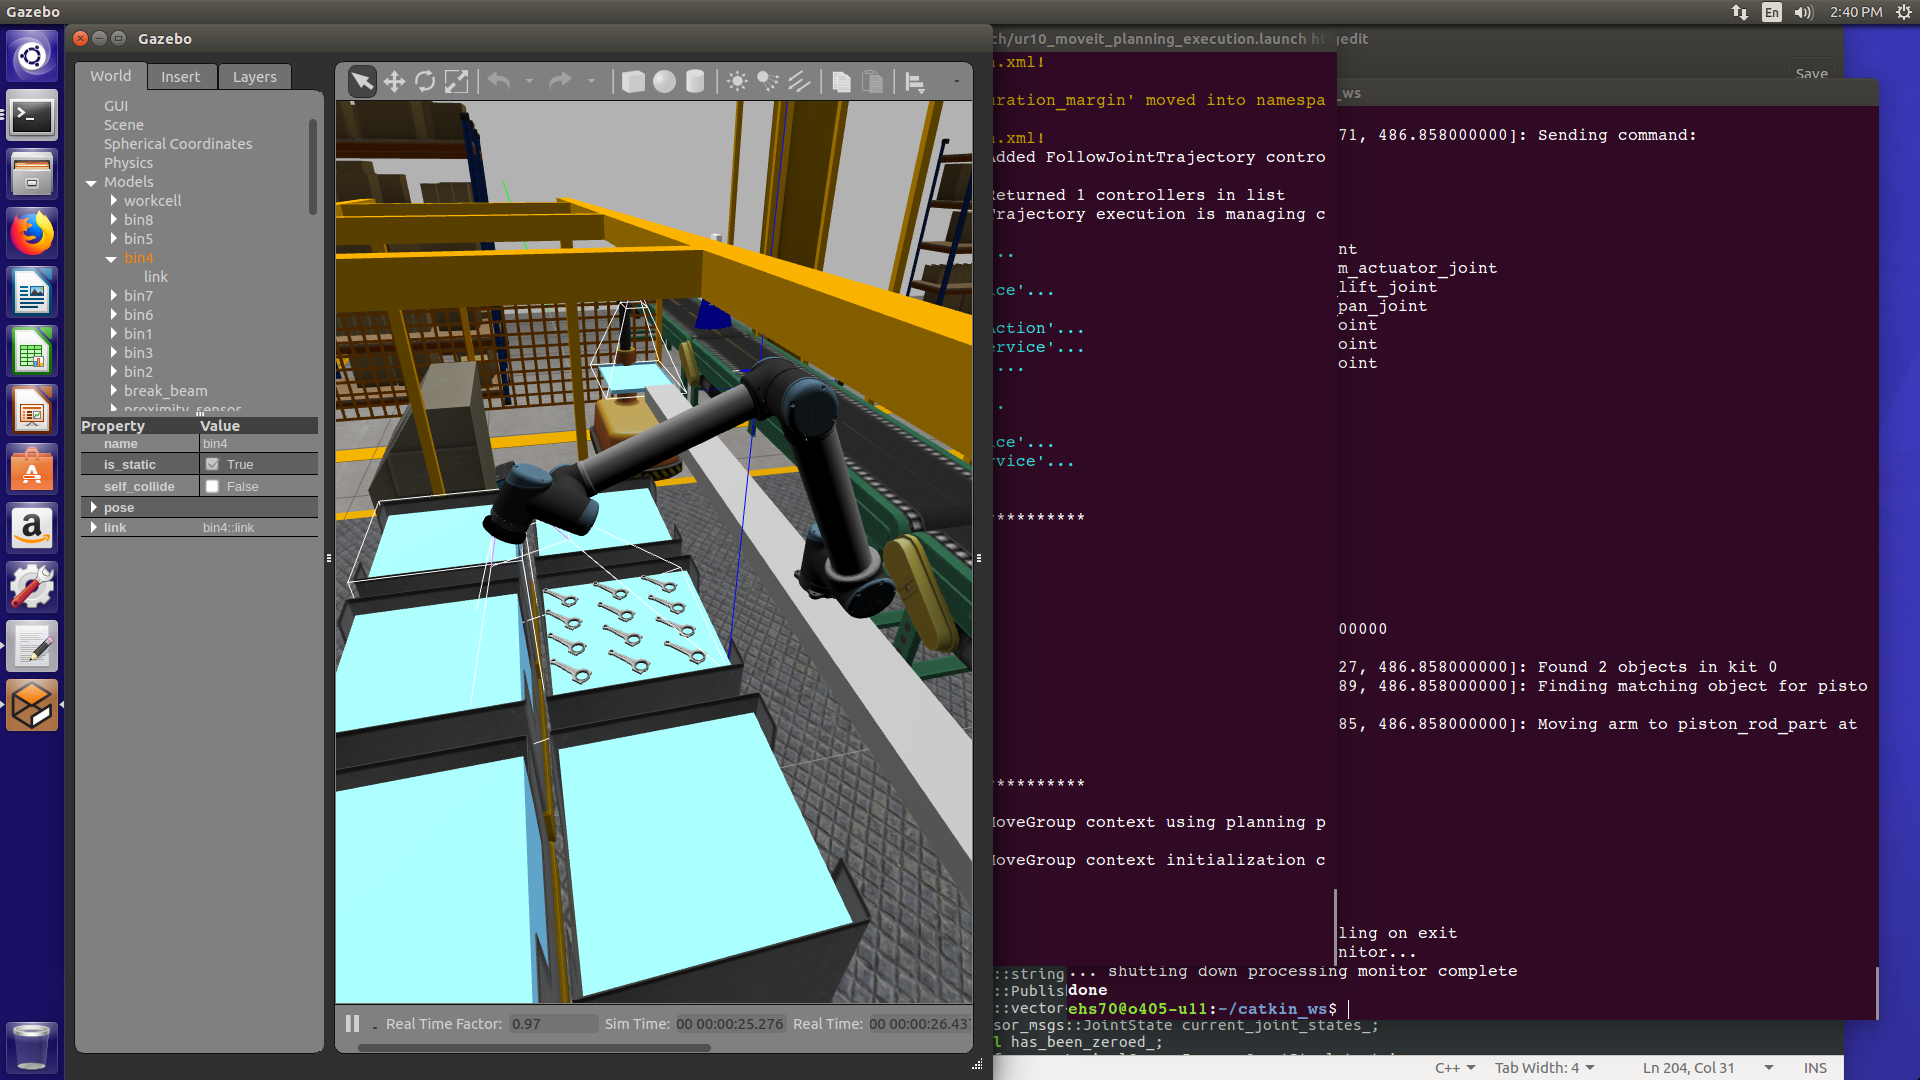
\includegraphics[scale=0.3,angle=270]{HW3_images/initial_config}
\end{center}{}
\newpage
After running our program:
\begin{center}
    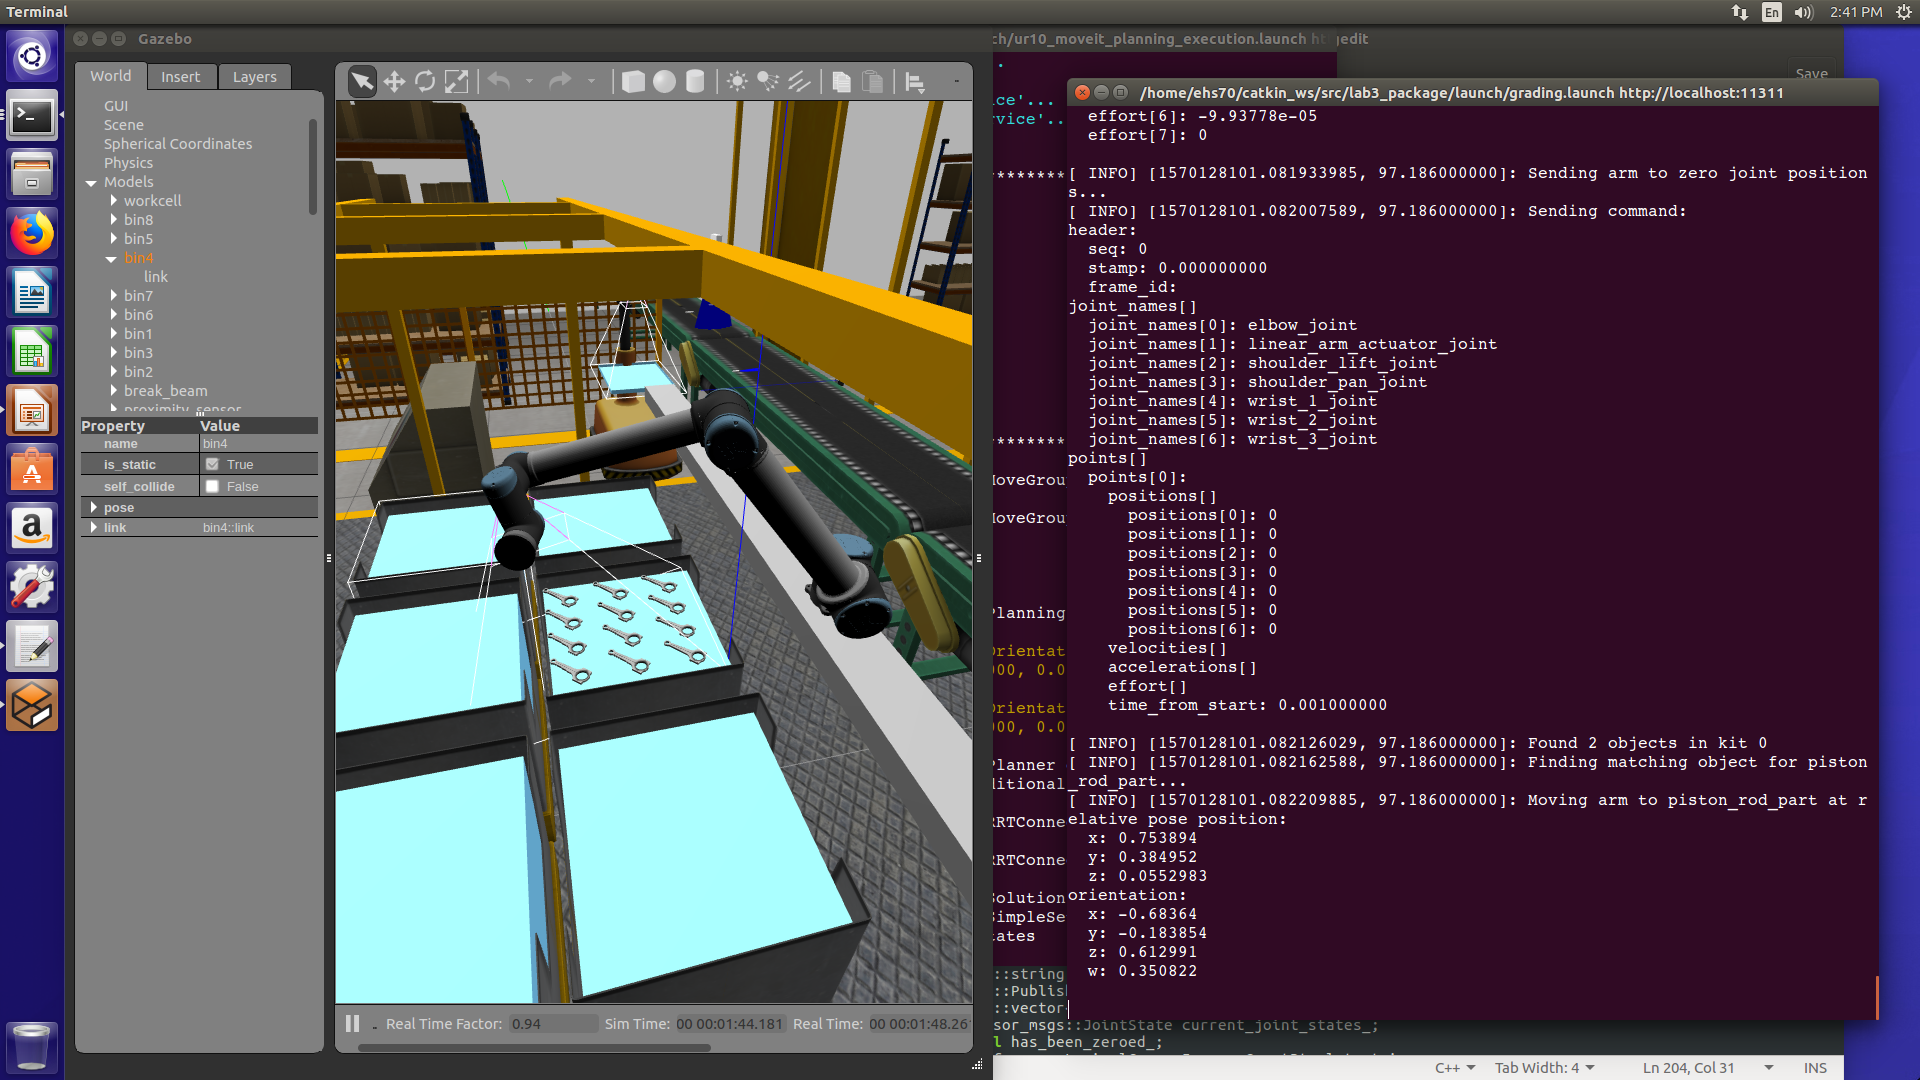
\includegraphics[scale=0.3,angle=270]{HW3_images/after_config}
\end{center}{}
\end{document}
